
%%%%%%%%%%%%%%%%%%%%%%% file adhocnow15_bolster.tex %%%%%%%%%%%%%%%
%[Ad Hoc Now 2015](http://www.netmode.ntua.gr/adhocnow2015/index.html)
%
%# Dates
%* Deadline: 7/2/15
%* Acceptance: 7/3/15
%* Due: 28/3/15
%* Dates: 29/6/15-2/7/15
%
%# Topics of Interest
%* Access Control 
%* Ad Hoc Networks of Autonomous Intelligent Systems 
%* Algorithmic Issues
%* Analytic Methods and Modeling for Performance Evaluation 
%* Ad Hoc Network Applications and Architectures 
%* Delay-Tolerant Networking
%* Distributed Algorithms for Ad Hoc Networks 
%* Energy Efficiency 
%* Geometric Graphs
%* Location Discovery and Management 
%* Mobility Handling and Utilization 
%* Wireless Mesh Networks
%* Big Data Inspired Data Sensing
%* Mobile Ad Hoc Computing Platforms
%* Systems and Testbeds 
%* Mobile Social Networking 
%* Quality-of-Service 
%* Routing Protocols (Unicast, Multicast, etc.) 
%* Secure Services and Protocols 
%* Sensor Networks 
%* Self-Configuration 
%* Service Discovery 
%* Timing Synchronization 
%* Vehicular Networks 
%* Wireless Internet
%* Processing and Networking Technologies Complexity and Computational Issues
%* Prototype systems and real-world deployment experiences
%
%# Proposed Area of Focus
%Re-present Bellas Chap 4 work with extensions to explain and explore differences between Ad Hoc and Marine.
%
%
%%%%%%%%%%%%%%%%%%%%%%%%%%%%%%%%%%%%%%%%%%%%%%%%%%%%%%%%%%%%%%%%%%%


\RequirePackage{snapshot}
\documentclass[runningheads,a4paper]{llncs}

\usepackage{amssymb}
\usepackage{amsmath}
\setcounter{tocdepth}{3}
\usepackage{graphicx}
\usepackage{float}

% Added to fix Table input
\usepackage{booktabs}
\usepackage{subcaption}

% Added to enhance todo lists, possibly need deleted pre pub
%\usepackage{todonotes}
\usepackage{hyperref}

\usepackage{url}
\newcommand{\keywords}[1]{\par\addvspace\baselineskip
\noindent\keywordname\enspace\ignorespaces#1}

\begin{document}

\mainmatter  % start of an individual contribution

% first the title is needed
\title{A Trust Framework for Autonomous Marine Communications Environments}

% a short form should be given in case it is too long for the running head
\titlerunning{A Trust Framework for Autonomous Marine Communications Environments}

% the name(s) of the author(s) follow(s) next
%
% NB: Chinese authors should write their first names(s) in front of
% their surnames. This ensures that the names appear correctly in
% the running heads and the author index.
%
\author{Andrew Bolster, Alan Marshall}
%
\authorrunning{A Trust Framework for Autonomous Marine Communications Environments}
% (feature abused for this document to repeat the title also on left hand pages)

% the affiliations are given next; don't give your e-mail address
% unless you accept that it will be published
\institute{Advanced Networks Research Group, \\Department of Electrical Engineering \& Electronics,\\
University of Liverpool, UK\\
\url{{andrew.bolster,alan.marshall}@liv.ac.uk}\\
\url{http://www.anrg.liv.ac.uk/}}

\maketitle   

\begin{abstract}
  This paper presents a Trust Management Framework (TMF) for Underwater Autonomous Networks. 
  We present a comparative study on the operation and performance of such trust frameworks between a typical terrestrial and the harsh underwater communications environment, examining the scaling factors involved (periodicity, physical spacing, etc.) in comparing and contrasting these environments. In this paper we demonstrate the need for a different approach towards metric selection and trust-timing in such constrained networks, and a performance comparison with a selection of current TMF assessment processes.
  \keywords{ad-hoc, MANET, trust, marine, underwater, acoustic}
\end{abstract}

\section{Introduction}\label{sec:introduction}

As mobile ad-hoc networks (MANETs) grow beyond the terrestrial arena, their operation and the protocols designed around them must be reviewed to assess their suitability to different communications environments, ensuring their continued security, reliability, and performance.

Trust Management Frameworks (TMFs) provide information to assist the estimation of future states and actions of nodes within networks.
This information is used to optimize the performance of a network against malicious, selfish, or defective misbehaviour by one or more nodes.
Previous research has established the advantages of implementing TMFs in 802.11 based MANETs, particularly in terms of preventing selfish operation in collaborative systems \cite{Li2007}, and maintaining throughput in the presence of malicious actors \cite{Buchegger2002}

Most current TMFs use a single type of observed action to derive trust values, i.e. successfully forwarded packets. These observations then inform future decisions of individual nodes, for example, route selection \cite{Li2008}.

Recent work has demonstrated use of a number of metrics to form a ``vector'' of trust.
The Multi-parameter Trust Framework for MANETs (MTFM)\cite{Guo11}, uses a range of physical metrics beyond packet delivery/loss rate (PLR) to form a vector of trust.
This vectorized trust allows a system to detect and identify the tactics being used to undermine or subvert trust.
To date this work has been limited to terrestrial, RF based networks, however as autonomous underwater vehicles (AUVs) become more capable, and economical, they are being used in many applications requiring trust.
These applications are using the collective behaviour of teams or fleets of these AUVs to accomplish tasks \cite{Caiti2011}.
With this use being increasingly isolated from stable communications networks, the establishment of trust between nodes is essential for the reliability and stability of such teams.
As such, the use of trust methods developed in the terrestrial MANET space must be re-appraised for application within the challenging underwater communications channel.

The paper is laid out as follows.
In Section \ref{sec:trustandtmfs} we discuss Trust and Trust Management Frameworks, defining our terminology and reviewing the justifications for the use and development of Trust Management Frameworks in marine acoustic networks.
In Section \ref{sec:marineacousticnetworks}, we review selected features of the underwater communications channel, highlighting particular challenges and differentials against terrestrial equivalents.
In Section \ref{sec:initialsystemcharacterization}, we establish an experimental configuration for the marine space, and review the scenarios and results presented in \cite{Guo11}.
In Section \ref{sec:trustresultsanddiscussion}, we present our findings in trust establishment and malicious behaviour detection, comparing with current TMFs such as OTMF and Beta.

The contributions of this paper are: A Trust Management Framework applicable to Underwater MANETs, a study on the comparative operation and performance between terrestrial and underwater MANETs using TMFs, and a review of metric suitability for Trust Management Frameworks in marine environments, informing future metric selection for experimenters and theorists.

\section{Trust and Trust Management Frameworks}\label{sec:trustandtmfs}

\subsection{Trust in MANETs}\label{sec:trustinmanets}

Trust is the level of confidence one agent has in another to perform an action. 
The distributed and dynamic nature of MANETs mean that it is difficult to maintain a trusted third party (TTP) or evidence based trust system such as Certificate Authorities (CA) or Public Key Infrastructure (PKI).
Distributed trust management frameworks aim to detect, identify, and mitigate the impacts of malicious actors by distributing per-node assessments and opinions to collectively self-police behaviour.
Various models and algorithms for describing trust and developing trust management in distributed systems, P2P communities or wireless networks have been considered.
Taking some examples;

\begin{itemize}
  \item \emph{The Objective Trust Management Framework} takes a Bayesian Beta function to model per-link Packet Loss Rate (PLR) over time, combining ``Trust'' and ``Confidence of Assessment'' into a single value \cite{Li2008}.
    OTMF however does not appropriately combat multi-node-collusion in the network \cite{Cho2011}.
  \item \emph{Trust-based Secure Routing}\cite{Moe2008a} demonstrated an extension to Dynamic Source Routing (DSR), incorporating a Hidden Markov Model of next-hop network, reducing the efficacy of Byzantine attacks such as black-hole routing.
  \item \emph{CONFIDANT}\cite{Buchegger2002} presented an approach using a probabilistic estimation of PLR, similar to OTMF, also introducing a topology weighting scheme that also weighted trust assessments based on historical experience of the reporter.
  \item \emph{Fuzzy Trust-Based Filtering}; \cite{Luo2008} presents the use of Fuzzy Inference to adapt to malicious recommenders using conditional similarity to classify performance with overlapping Fuzzy Set Membership, filtering assessments across a network.
\end{itemize}

These TMFs can be generalised as single-value probabilistic estimation, based around using a binary input state and generating an probabilistic estimation of the future states of that input. This expectation value is $\text{beta}(p|\alpha,\beta) \to E(p) = \frac{\alpha}{\alpha+\beta}$ where $\alpha$ and $\beta$ represent the number of successful and unsuccessful interactions respectively.

These single metric TMFs provide malicious actors with a significant advantage if their activity is undetectable by that metric.
In the case where the attacker can subvert the TMF, the metric under assessment by that TMF does not cover the threat mounted by the attacker.
In turn, this causes a super-linearly negative effect in the efficiency of the network, as the TMF is assumed to have reduced the possible set of attacks when it has actually made it more advantageous to attack a different part of the networks operation.
An example of such a situation would be in a TMF focused on PLR where an attacker selectively delays packets going through it, reducing overall throughput but not dropping any packets.
Such behaviour would not be detected by the TMF.

There are also situations where the observed metrics will include significant noise and occur at irregular, sparse, intervals.
Conventional approaches such as probabilistic estimation do not produce trust values that reflect the underlying reality and context of the metrics available, as they require a-priori assumption that the trust value under exploration has an expected distribution, that distribution is mono-modal, and the input metrics are binary.
In scenarios with variable, sparse, noisy metrics, estimating the distribution is difficult to accomplish a-priori.

\subsection{Grey Theory and MTFM}

Grey Theory performs cohort based normalization of metrics at runtime. 
This creates a more stable contextual assessment of trust, providing a ``grade'' of trust compared to other observed nodes in that interval, while maintaining the ability to reduce trust values down to a stable assessment range for decision support without requiring every environment entered into to be characterised.
This presents a stark difference between the Grey and Probabilistic approaches.
Grey assessments are relative in both fairly and unfairly operating networks.
Nodes will receive mid-range trust assessments if there are no malicious actors as there is no-one else ``bad'' to compare against, and variations in assessment will be primarily driven by topological and environmental factors.

Guo\cite{Guo11} demonstrated the ability of Grey Relational Analysis (GRA)\cite{Zuo1995} to normalise and combine disparate traits of a communications link such as instantaneous throughput, received signal strength, etc. into a Grey Relational Coefficient, or a ``trust vector''.

In the case of the terrestrial communications network used in \cite{Guo11}, the observed metric set $X = {x_1,\dots,x_M}$ representing the measurements taken by each node of its neighbours at least interval, is defined as $X=[$packet loss rate, signal strength, data rate, delay, throughput$]$.
The trust vector is given as
%
\begin{align}
  \label{eq:grc}
  \theta_{k,j}^t = \frac{\min_k|a_{k,j}^t - g_j^t| + \rho \max_k|a_{k,j}^t-g_j^t|}{|a_{k,j}^t-g_j^t| + \rho \max_k|a_{k,j}^t-g_j^t|} \\
  \phi_{k,j}^t = \frac{\min_k|a_{k,j}^t - b_j^t| + \rho \max_k|a_{k,j}^t-b_j^t|}{|a_{k,j}^t-b_j^t| + \rho \max_k|a_{k,j}^t-b_j^t|} \notag 
\end{align}
%
where $a_{k,j}^t$ is the value of a observed metric $x_j$ for a given node $k$ at time $t$, $\rho$ is a distinguishing coefficient set to $0.5$, $g$ and $b$ are respectively the '``good'' and ``bad'' reference metric sequences from $\{a_{k,j}^t k=1,2\dots K\}$, e.g. $g_j=\max_k({a_{k,j}^t})$,  $b_j=\min_k({a_{k,j}^t})$ (where each metric is selected to be monotonically positive for trust assessment, e.g. higher throughput is always better). 

Weighting can be applied before generating a scalar value which allows the identification and classification of untrustworthy behaviours.

%
\begin{equation}
  \label{eq:metric_weighting}
  [\theta_k^t, \phi_k^t] = \left[\sum_{j=0}^M h_j \theta_{k,j}^t,\sum_{j=0}^M h_j \phi_{k,j}^t \right]
\end{equation}
Where $H=[h_0\dots h_M]$ is a metric weighting vector such that $\sum h_j = 1$, and in the basic case, $H=[\frac{1}{M},\frac{1}{M}\dots\frac{1}{M}]$ to treat all metrics evenly.
$\theta$ and $\phi$ are then scaled to $[0,1]$ using the mapping $y = 1.5 x - 0.5$.
The $[\theta,\phi]$ values are reduced into a scalar trust value by $T_k^t = ({1+{(\phi_k^t)^2}/{(\theta_k^t)^2}})^{-1}$.
This trust value minimises the uncertainties of belonging to either best ($g$) or worst ($b$) sequences in \eqref{eq:grc}.

MTFM combines this GRA with a topology-aware weighting scheme\eqref{eq:networkeffects} and a fuzzy whitenization model\eqref{eq:whitenization}. There are three classes of topological trust relationship used; Direct, Recommendation, and Indirect.
Where an observing node, $n_i$, assesses the trust of another, target, node, $n_j$; the Direct relationship is $n_i$'s own observations $n_j$'s behaviour.
In the Recommendation case, a node $n_k$, which shares Direct relationships with both $n_i$ and $n_j$, gives its assessment of $n_j$ to $n_i$.
The Indirect case, similar to the Recommendation case, the recommender $n_k$, does not have a direct link with the observer $n_i$ but $n_k$ has a Direct link with the target node, $n_j$.
These relationships give us node sets, $N_R$ and $N_I$ containing the nodes that have recommendation or indirect, relationships to the observing node respectively.
%
\begin{align}
  \label{eq:networkeffects}
  T_{i,j}^{MTFM}=\frac{1}{2} \cdot \max_s\{f_s(T_{i,j})\} T_{i,j}+&\frac{1}{2} \frac{2|N_R| }{2|N_R| + |N_I|}\sum_{n \in N_R} \max_s\{f_s(T_{i,n})\} T_{i,n}\\ \notag
  +&\frac{1}{2} \frac{|N_I| }{2|N_R| + |N_I|}\sum_{n \in N_I} \max_s\{f_s(T_{i,n})\} T_{i,n} 
\end{align}
 Where $T_{i,n}$ is the subjective trust assessment of $n_i$ by $n_n$, and $f_s = [ f_1,f_2, f_3]$ given as:
\begin{align}
  \label{eq:whitenization}
  f_1(x)&= -x+1\notag\\
  f_2(x)&= 
  \begin{cases}
    2x & \text{if }x\leq 0.5\\
    -2x+2 & \text{if }x>0.5
  \end{cases}\\
  f_3(x)&= x\notag
\end{align}
%
\section{Marine Acoustic Networks}\label{sec:marineacousticnetworks}

The key challenges of underwater acoustic communications are centred around the impact of slow and differential propagation of energy (RF, Optical, Acoustic) through water, and it's interfaces with the seabed / air.
The resultant challenges include; long delays due to propagation, significant inter-symbol interference and Doppler spreading, fast and slow fading due to environmental effects (aquatic flora/fauna; surface weather), carrier-frequency dependent signal attenuation, multipath caused by the medium interfaces, variations in propagation speed due to depth dependant effects (salinity, temperature, and pressure), and subsequent refractive spreading and lensing due to that same propagation variation\cite{Partan2006}.

The attenuation that occurs in an underwater acoustic channel over a distance $d$ for a signal about frequency $f$ in linear power as $A_{\text{aco}}(d,f) = A_0d^ka(f)^d$ and in $dB$ form is given as 
%
\begin{equation}
  \label{eq:acoattenuationdb}
  10 \log A_{\text{aco}}(d,f)/A_0 = k \cdot 10 \log d + d \cdot 10 \log a(f)
\end{equation}
%
where $A_0$ is a unit-normalising constant, $k$ is a spreading factor (commonly taken as 1.5), and $a(f)$ is the absorption coefficient, expressed empirically using Thorp's formula \eqref{eq:thorp} from \cite{Stojanovic2007}
%
\begin{equation}
  \label{eq:thorp}
  10 \log a(f) = 0.11 \cdot \frac{f^2}{1+f^2} + 44\cdot\frac{f^2}{4100+f^2}+ 2.75\times10^{-4} f^2 + 0.003
\end{equation}
%
Refractive lensing and the multipath nature of the medium result in supposedly line of sight propagation being extremely unreliable for estimating distances to targets.
The first arriving beam has as the very least bent in the medium, and commonly has reflected off the surface/seabed before arriving at a receiver, creating secondary paths that are sometimes many times longer than the first arrival path, generating symbol spreading over orders of seconds depending on the ranges and depths involved.
Extensive Forward Error Correction coding is used on such channels to minimise packet losses.

Comparing $A_{aco}(d,f)$ with the RF Free-Space Path Loss model $A_{\text{RF}}(d,f) \approx \left( \frac{4\pi d f}{c} \right)^2$, the impact of range on signal power is exponential underwater, rather than quadratic in RF space ($A_{\text{aco}} \propto f^{2d}$ vs $A_{\text{RF}} \propto (df)^2$). 
While both frequency dependant factors are quadratic, approximating the factors in \eqref{eq:thorp}, $f\propto A_{\text{aco}}$ is at least 4 orders of magnitude higher than $f\propto A_{\text{RF}}$


\subsection{Trust in Marine Networks}\label{sec:trust_in_marine}

With demand for smaller, more decentralised marine survey and monitoring systems, and a drive towards lower per-unit cost, TMFs are going to be increasingly applied to the marine space, as the benefits they present are significant.
Beyond the constraints of the communications environment, knock on pressures are applying in battery capacity, on-board processing, and locomotion.
These pressures simultaneously present opportunities and incentives for malicious or selfish actors to appear to cooperate while not reciprocating, in order to conserve power for instance.
These multiple aspects of potential incentives, trust, and fairness do not directly fall under the scope of single metric trusts discussed above, and this context indicates that a multi-metric approach may be more appropriate.


\section{Initial System Model Characterization}\label{sec:initialsystemcharacterization}

\subsection{Mobility, Topology, and Communications}

Four mobility scenarios were used in \cite{Guo11} to explore trust behaviour; all nodes static, a central node $n_1$ performing a random walk with other nodes remaining static, all nodes but the central node ($n_1$) randomly walking, and all nodes randomly walking. From these we select the all static and all mobile cases for presentation.
The reason for this is that giving a malicious node special privilege or capabilities will skew the results of trust assessment, as the behaviours of the static and mobile nodes will be significantly different regardless of malice.

The six nodes are placed as in \cite{Guo11}, as per Fig.~\ref{fig:s1_layout}, with each node on average 100m from each other, as per \cite{Guo11}.
The use of six nodes and the particular layout enables the investigation of the three trust relationships based on minimum path topologies, such that the node generating the trust assessments, $n_0$ has Direct, Recommendation, and Indirect trust assessments of $n_1$ available to it from itself, $[n_2,n_3]$, and $[n_4,n_5]$ respectively.

In all of the scenarios, each link from $n_i \rightarrow n_j$ periodically sent 10 second bursts of Constant Bit Rate (CBR) style traffic.
%
\begin{figure}[h]
  \centering
  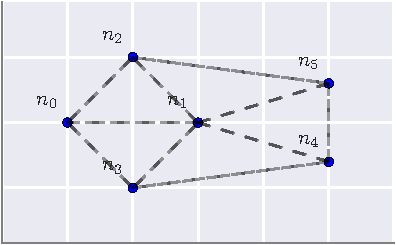
\includegraphics[width=0.3\textwidth]{img/s1_layout.pdf}
  \caption{Initial layout with nodes spaced an average of 100m apart}
  \label{fig:s1_layout}
\end{figure}
%
Guo demonstrated that when compared against OTMF and Beta trust assessment, MTFM provided increased variation in trust assessment over time, providing more information about the nodes behaviour than packet delivery probability. 
By weighting the metrics used in MTFM, it was shown that the trust assessments could be used to identify the style of misbehaviour being performed within the network and by who.
We present a corollary method to investigate and apply this work to the Marine MANET field.

\subsection{Simulation Background}

Simulations were conducted using a Python based simulation framework, SimPy\cite{Mueller2003SimPy}, with a network stack built upon AUVNetSim\cite{Miquel2008}, with transmission parameters (Table \ref{tab:sysconstraints}) taken from and validated against \cite{Stojanovic2007} and \cite{Stefanov2011}.

Given the differences in delay and propagation between RF and marine networks, it is natural that the same application rates (e.g. packet emission rates or throughput) and node separations should not be assumed to be equivalent.
Therefore, we characterise an operational zone of performance within which the network can operate stably.
%
\begin{table}[h]
  \caption{Comparison of system model constraints as applied between Terrestrial and Marine communications} \label{tab:sysconstraints}
  \begin{center}
    \setlength{\tabcolsep}{8pt}
    \begin{tabular}{lccc}
      \toprule
      Parameter & Unit & Terrestrial & Marine \\
      \midrule
      Simulated Duration & $s$ & 300 & 18000\\
      Trust Sampling Period & $s$ & 1 & 600 \\
      Simulated Area & $km^2$ & 0.7 & 0.7-4 \\
      Transmission Range & $km$ & 0.25 & 1.5 \\
      Physical Layer & & RF(802.11) & Acoustic\\
      Propagation Speed& $m/s$ & $3\times10^8$ & 1490\\
      Center Frequency& $Hz$ & $2.6\times10^9$ & $2 \times 10^4$ \\
      Bandwidth& $Hz$ & $22\times10^6$ & $1\times10^4$\\
      MAC Type & & CSMA/DCF & CSMA/CA\\
      Routing Protocol & & DSDV & FBR \\
      Max Speed & $ms^{-1}$ & 5 & 1.5 \\
      Max Data Rate & $bps$ & $5\times10^6$ & $\approx 240$ \\
      Packet Size & bits & 4096 &  9600 \\
      Single Transmission Duration & $s$ & 10 & 32 \\
      Single Transmission Size & bits & $10^7$ & $9600$ \\
      \bottomrule
    \end{tabular}
    \setlength{\tabcolsep}{6pt}
  \end{center}
\end{table}
%
\subsection{Scaling Considerations between Terrestrial and Underwater Environments}

In this section we characterise the simulated communications environment, establishing an optimal packet emission rate for comparison against \cite{Guo11}.

We establish a appropriate safe operating zone for marine communications by looking at the communications rate and physical distribution factors across the two selected mobility scenarios.
In scaling the physical distribution of the nodes, we also scale the environment in which the nodes are restricted to, which has a significant impact on the number of potential runtime topologies, with nodes getting increasingly isolated as the environment space increases.
This leads to increasing delays as routes are constantly broken, re-advertised and re-established. 
From Table~\ref{tab:sysconstraints}, the operating transmission range of this model of acoustic communications is $\approx 6$ times further than that of 802.11, indicating that a suitable operating environment will have an area $\approx \sqrt{6}$ times the area of the 802.11 case.
However, it was recognised in Section~\ref{sec:marineacousticnetworks} that the relationship between attenuation and distance is exponential underwater, so this would represent an upper bound of performance, where nodes begin approximately 400$m$ apart. 

As the separation is increased, the emission rate at which the network becomes saturated decreases, reducing overall throughput. 
This throughput degradation is tightly coupled with the mobility.
For instance, in Fig.~\ref{fig:throughput_static}, where all nodes are static, we do not see significant drops in saturation rates until we approach 800m, nearly double our initial estimate. 
However, in Fig. ~\ref{fig:throughput_all_mobile}, where all the nodes are randomly walking, the saturation point collapses from 0.025pps at 300m to 0.015pps at 400m.
These results indicate that the best area to continue operating in for a range of node separations is at 0.015pps, and that a reasonable position scaling is from 100m to 300m, beyond which communication becomes increasingly unstable, especially in terms of end to end delay (not shown) 
%
\begin{figure}[h]
\begin{subfigure}{.5\textwidth}
  \centering
  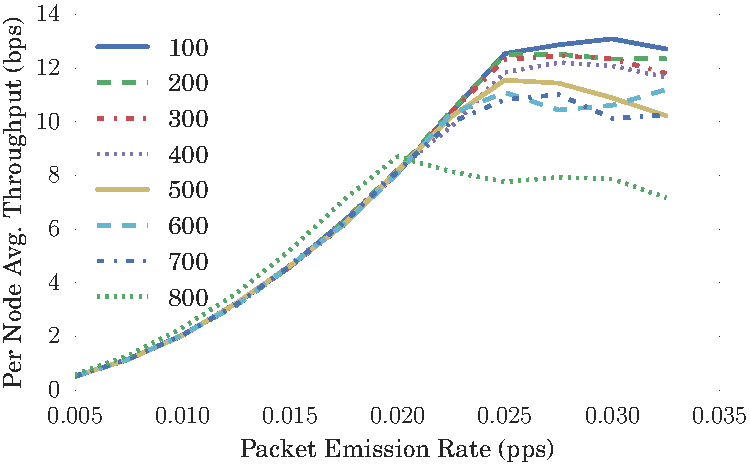
\includegraphics[width=.9\linewidth]{img/throughput_sep_lines_static.pdf}
  \caption{Static}
  \label{fig:throughput_static}
\end{subfigure}%
\begin{subfigure}{.5\textwidth}
\centering
  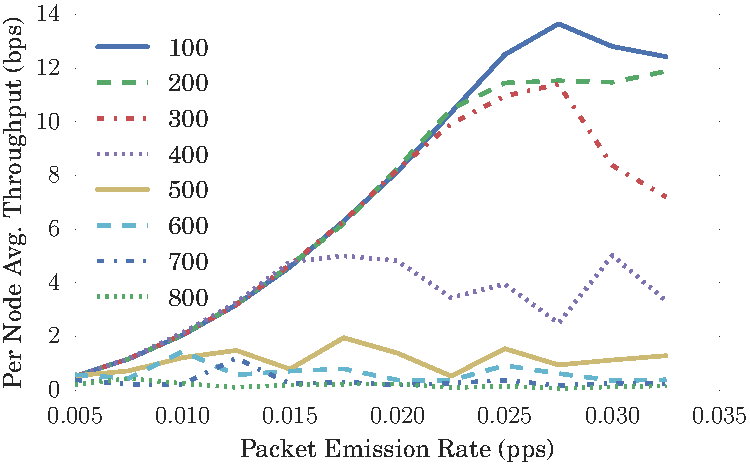
\includegraphics[width=.9\linewidth]{img/throughput_sep_lines_all_mobile.pdf}
  \caption{Mobile}
  \label{fig:throughput_all_mobile}
\end{subfigure}
\caption{Throughput Characteristics for varying node separations across increasing packet emission rates}
\label{fig:scenario_throughputs_plain}
\end{figure}
%
\section{Trust}\label{sec:trustresultsanddiscussion}

Having established a safe operating range for comparison, at 300m separation and an emission rate of 0.015pps, we repeat the static and mobile scenarios presented in \cite{Guo11}. We select an assessment period of 10 mins for a 5 hour mission to scale in comparison to relative bitrates experienced (1Mbps vs $\approx15$bps).

Metrics used for Grey assessment are transmitted and received throughput and power, delay, and packet loss rate as calculated by aborted, unacknowledged, transmissions.
Compared to \cite{Guo11}, this metric set lacks a data rate quantity as the network is not dynamically adjusting bandwidth.
In context of Grey Relational Coefficient generation \eqref{eq:grc}, the best sequence $g$ was selected using the lowest PLR, delay, and powers, and the highest throughputs, with the worst sequence, $b$ the inverse of these metrics.

The particular factors under discussion are the relative performance of MTFM against OTMF and Beta with respect to statistical stability across mobilities and in responsiveness to changing network behaviour. 
We establish a similar result set by initially tracking the resultant trust values established by MTFM in the pair of mobility scenarios, shown in Fig.\ref{fig:trust_mobility}.
For simplicity, we are primarily concerned with the observational trust relationship between $n_0$ and $n_1$, i.e. $n_0$'s assessment of the trustworthiness of $n_1$, or $T_{1,0}$.
We are also concerned with the opinions of $n_1$ provided to $n_0$ by other nodes, where $[T_{1,2},T_{1,3}]$ and $[T_{1,4},T_{1,5}]$ denote the sets of recommendation and indirect trust assessment respectively.
We also include aggregate assessments; $T_{1,\text{Avg}}$, the flat average of direct trust assessments of $n_1$, $T_{1,\text{Net}}$, that weights assessments according to the network topology from \eqref{eq:networkeffects}, without the whitenization factor $f_s$, and $T_{1,\text{MTFM}}$, the final MTFM trust assessment value based on both network topology and whitenization from \eqref{eq:whitenization}.

The variability in assessment is loosely tied to the mobility; in the static case (Fig.~\ref{fig:trust_static}), we see that the nodes close to $n_1$ ($[n_0,n_2,n_3]$) have reasonably consistent distributions, and as the range increases out to $[n_4,n_5]$, this variability increases.
In the full mobility case, shown in Fig.~\ref{fig:trust_all_mobile}, this subjective variability is greatly increased. 
As the topology is highly dynamic, delays due to re-establishing routes can be very large, perturbing the trust value.
The aggregate trust values using topology information ($iT_{1,\text{Net}},T_{1,\text{MTFM}}$) display a decreased variation than those of the individual subjective observations in both cases.
%
\begin{figure}[h]
\begin{subfigure}{.5\textwidth}
  \centering
  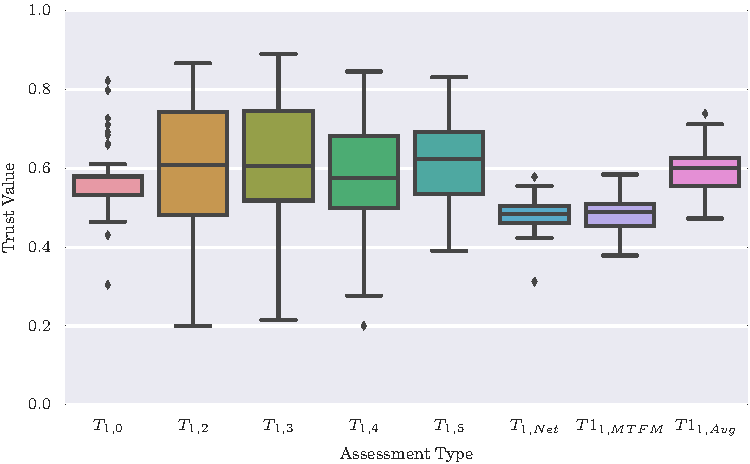
\includegraphics[width=\linewidth]{img/trust_bella_static.pdf}
  \caption{Static}
  \label{fig:trust_static}
\end{subfigure}%
\begin{subfigure}{.5\textwidth}
\centering
  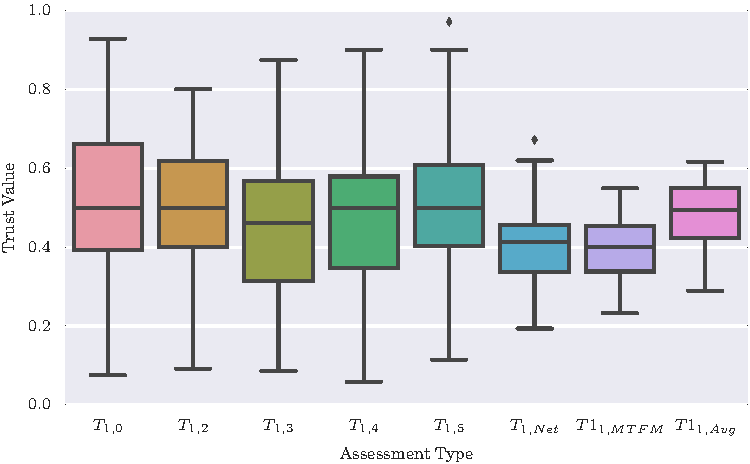
\includegraphics[width=\linewidth]{img/trust_bella_all_mobile.pdf}
  \caption{Mobile}
  \label{fig:trust_all_mobile}
\end{subfigure}
\caption{MTFM Trust assessments of $n_1$ ($T_{1,X}$)\protect\footnotemark}
\label{fig:trust_mobility}
\end{figure}
%
\subsection{Comparison under malicious behaviour}

Guo introduces a range of malicious actors, including modification of the packet loss rate of routing nodes and limiting throughput on a per-link basis as well as a selection of combined misbehaviours. 

Given that the established links are already heavily constrained, heavy handed attacks such as introducing selective PLR and adding to the already extreme and hugely variable delays would severely impact the general performance of the network beyond the scope of simple selfishness, effectively triggering saturation collapses in regions that the network should be stable.
Therefore, we select a Selfish Power Control behaviour, where $n_1$ increases it's transmission power by 20\% for all nodes \emph{except} communications with $n_0$.

In order to assess this experiment, parallel simulations were performed where there was no malicious behaviour, the ``fair'' scenario. 
From this, we apply a sequence of metric vectors that preferentially weight each metric during \eqref{eq:metric_weighting}.
For an arbitrary metric weight vector $H$, where the metric $m_j$ is emphasised as being twice as important as the other metrics, we form an initial weighting vector $H'=[h_i...h_M]$ such that $h_i = 1 \forall i \ne j; h_j=2$. We then scale that vector $H'$ such that $\sum H = 1$ by $H= \frac{H'}{\sum H'}$.
%Footnote for fig:trust_all_mobile
\footnotetext{Box plots centres indicate the median, bounds indicate the 25\%-75\% range, and whiskers represent the points within $\pm2\sigma$}
Using this process we can extract and highlight the primary aspects of an attack by comparing against the deviation from the 'fairness' set; 

\begin{figure}[h]
\begin{subfigure}{0.5\textwidth}
  \centering
  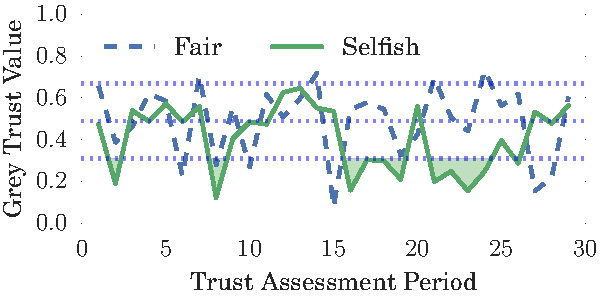
\includegraphics[width=.95\linewidth]{img/trust_bella_static_emph_ADelay_BadMouthingPowerControl.pdf}
  \caption{Delay}
  \label{fig:static_badmouthing_delay}
\end{subfigure}
\begin{subfigure}{0.5\textwidth}
\centering
  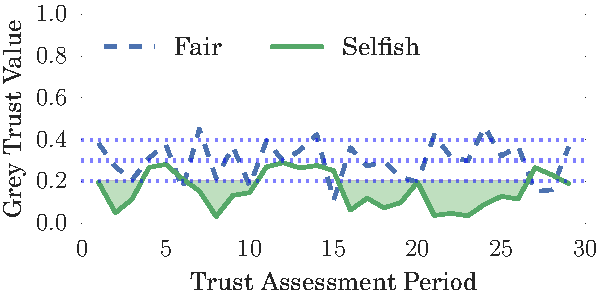
\includegraphics[width=.95\linewidth]{img/trust_bella_static_emph_ATXP_BadMouthingPowerControl.pdf}
  \caption{TX Power}
  \label{fig:static_badmouthing_txp}
\end{subfigure}
\begin{subfigure}{0.5\textwidth}
\centering
  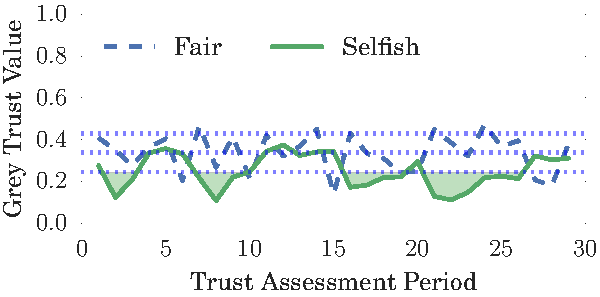
\includegraphics[width=.95\linewidth]{img/trust_bella_static_emph_RXThroughput_BadMouthingPowerControl.pdf}
  \caption{RX Throughput}
  \label{fig:static_badmouthing_rxthroughput}
\end{subfigure}
\begin{subfigure}{0.5\textwidth}
\centering
  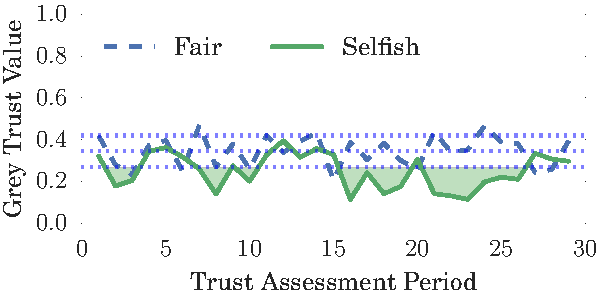
\includegraphics[width=.95\linewidth]{img/trust_bella_static_emph_TXThroughput_BadMouthingPowerControl.pdf}
  \caption{TX Throughput}
  \label{fig:static_badmouthing_txthroughput}
\end{subfigure}
\caption{$T_{1,MTFM}$ in the All Static case for the Selective Power Control behaviour, emphasising selected metrics and showing the mean and $\pm \sigma$ of $T_{1,MTFM}$ in the same 'fair' scenario}
\label{fig:static_badmouthing}
\end{figure}
%
\begin{figure}
\begin{subfigure}{0.5\textwidth}
  \centering
  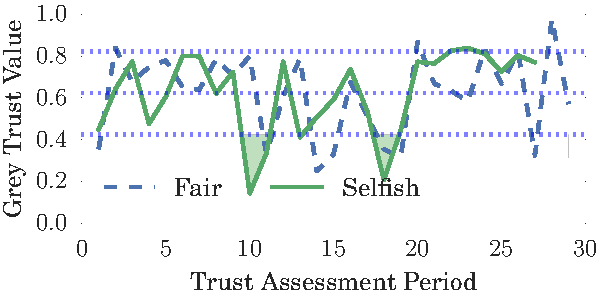
\includegraphics[width=.95\linewidth]{img/trust_bella_all_mobile_emph_ARXP_BadMouthingPowerControl.pdf}
  \caption{RX Power}
  \label{fig:all_mobile_badmouthing_rxp}
\end{subfigure}
\begin{subfigure}{0.5\textwidth}
\centering
  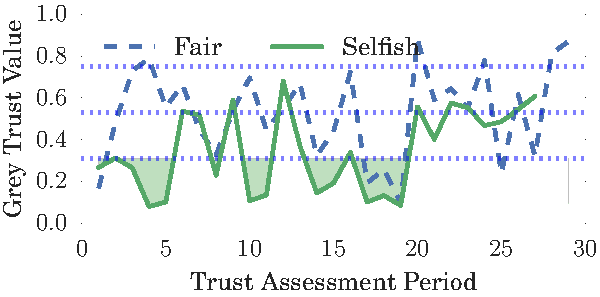
\includegraphics[width=.95\linewidth]{img/trust_bella_all_mobile_emph_ATXP_BadMouthingPowerControl.pdf}
  \caption{TX Power}
  \label{fig:all_mobile_badmouthing_txp}
\end{subfigure}
\begin{subfigure}{0.5\textwidth}
\centering
  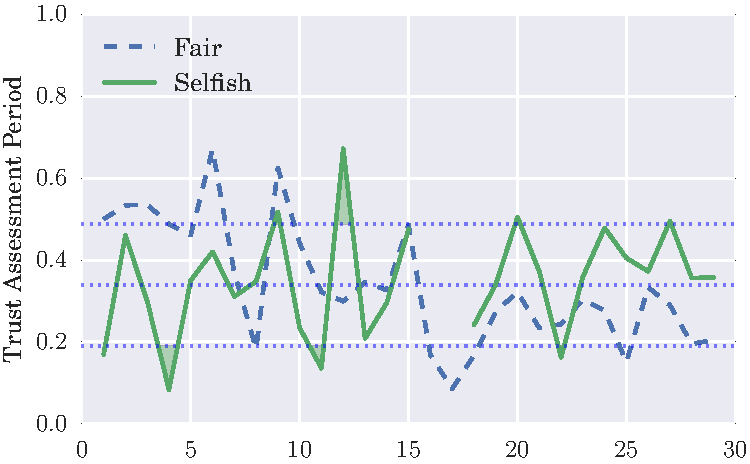
\includegraphics[width=.95\linewidth]{img/trust_bella_all_mobile_emph_RXThroughput_BadMouthingPowerControl.pdf}
  \caption{RX Throughput}
  \label{fig:all_mobile_badmouthing_rxthroughput}
\end{subfigure}
\begin{subfigure}{0.5\textwidth}
\centering
  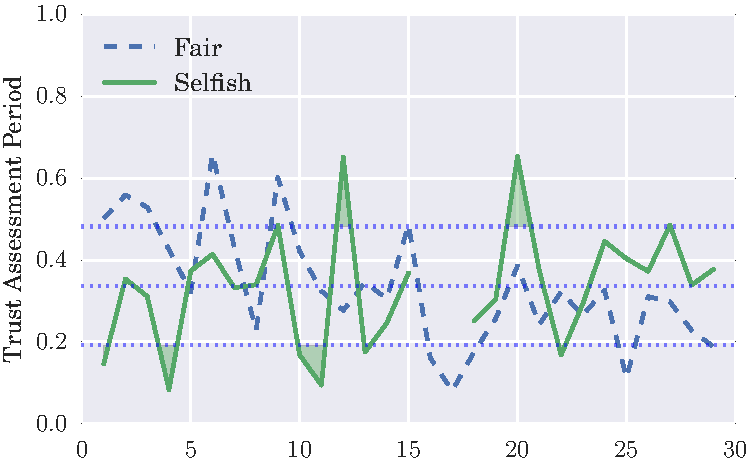
\includegraphics[width=.95\linewidth]{img/trust_bella_all_mobile_emph_TXThroughput_BadMouthingPowerControl.pdf}
  \caption{TX Throughput}
  \label{fig:all_mobile_badmouthing_txthroughput}
\end{subfigure}
\caption{$T_{1,MTFM}$ in the All Mobile case for the Selective Power Control behaviour}
\label{fig:all_mobile_badmouthing}
\end{figure}
%
From Fig.~\ref{fig:static_badmouthing} we can see that the selfish node is consistently outside the $\pm\sigma$ envelope of the fair comparison, particularly TX Power, with smaller impacts on RX/TX Throughput, as would be expected for a power related selfish behaviour. 
However, the impact on delay is minimal to insignificant, occasionally breaching the envelope for a short period. 
This was to be expected in a contention-based medium access network operating close to its saturation point; it can be observed that the delay deviance appears to increase as simulation time progresses. 
This indicates that the variation in delay could be caused not by a malicious behaviour but simple congestion.
In the mobile case (Fig.~\ref{fig:all_mobile_badmouthing}) we observe a similar pattern, however it should be noted that the deviation envelop is greatly increased compared to the static case due to the underlying variations in topology and configuration in this scenario.

A significant factor of trust assessment in such a constrained environment is that there may be long periods where two edge nodes (for instance, $n0 \to n_5$) may not interact at all. 
This can be due to a range of factors beyond potential malicious behaviour including simple random scheduling coincidence, and intermediate or neighbouring nodes collectively causing long back-off or contention periods.
This disconnection hinders trust assessment in two ways; assessing nodes that do not receive timely recommendations may make decisions based on very old data, and malicious nodes have a long dwelling time where they can operate under a reasonable certainty that the TMF will not detect it (especially if the node itself is behaving disruptively).
One potential solution to this would be to move from a stepping-window of trust periods to a continuous trust log, updated on packet reception rather than waiting for a number of packets to arrive.

In comparison to \cite{Guo11}, these results are qualitatively similar, however in this case the weighted deltas are significantly less clear than in the comparable terrestrial space, where Guo shows the same type of malicious behaviour and demonstrates a weighted delta from $\approx$ 0.4 to $\approx$ 0.9 across the simulation period, compared to our maximum delta in TX Power of $\approx$ 0.3 for an inconsistent interval.


\subsection{Comparison to OTMF and Beta}

The same experiments were also performed utilising OTMF and Beta assessment as well as MTFM, providing like-for-like comparison of assessment at runtime.
%
\begin{figure}[h]
  \begin{subfigure}{0.5\textwidth}
    \centering
    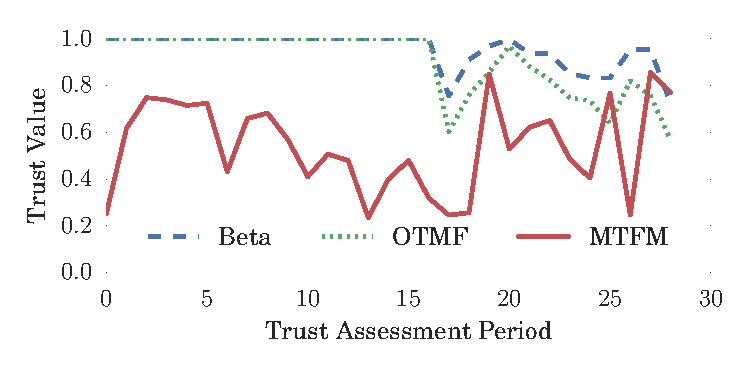
\includegraphics[width=.95\linewidth]{img/trust_beta_otmf_fair.pdf}
    \caption{Fair Scenario}
    \label{fig:all_mobile_fair_beta}
  \end{subfigure}
  \begin{subfigure}{0.5\textwidth}
    \centering
    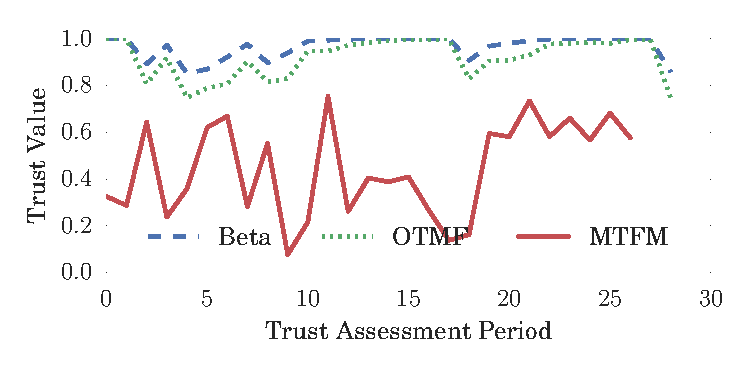
\includegraphics[width=.95\linewidth]{img/trust_beta_otmf_malicious.pdf}
    \caption{Selective Power Control scenario}
    \label{fig:all_mobile_badmouthing_beta}
  \end{subfigure}
\caption{$T_{1,0}$ for Beta, OTMF and MTFM assessment values for fair and selfish behaviours in the fully mobile scenario}
\label{fig:otmf_beta_comparison}
\end{figure}
%
The use of Forward Beam Routing and a CSMA/CA MAC scheme from AUVNetSim\cite{Miquel2008} in our simulation mitigates a significant number of packet losses through collision avoidance, and contention handling, leading to the situation that the only genuinely lost packets occur when a node moves completely out of range of any other node and times out in route discovery rather than transmission.
As such, confirmed packet losses are extremely rare and in a delaying network like this, it is difficult to set a differentiating time-out between packets that are in the network but queued, and packets that are actually 'lost'.
This renders OTMF and Beta assessment at best uninformative and at worst misleading; consistently providing nodes a high trust assessment as they have very little information to extract trust from. 
The single metric TMFs used in Terrestrial MANETs require regular and constant streams of positive and negative validation to shape and adjust their evaluations, which for a network with significant delays such as this, is not practical.

Fig.~\ref{fig:otmf_beta_comparison} shows a comparison between the unweighted response of MTFM compared to OTMF and Beta assessment functions on the same data for the fair and selfish behaviours respectively.
It is important to note a distinction between the expectations of MTFM compared to other TMFs; MTFM is primarily concerned with the identification of differences in the behaviours of nodes in a network, and is relative rather than absolute.
That is to say that under MTFM, agents are compared against the worst current performances across metrics of other nodes and graded against them, rather than the absolute (objective) approach taken by many TMFs.
This relative versus absolute difference is particularly clear when comparing mobility models. 
In this case, particularly since the method of attack was not directly related to PLR, OTMF and Beta have not registered significant activity in the correct behaviour.

While the MTFM value does not display any immediate difference between the two behaviours, we have shown that by exploring the metric space by weight variation, the existence and nature of the malicious behaviour can be discovered.
Another difference is that computationally, MTFM is significantly more intensive than the relatively simple Beta / OTMF algorithm, and the repeated metric matrix re-weighting required for real time behaviour detection is an area that requires optimization. 
As such, a hybrid system could be implemented, that used OTMF as a 'trigger' to detect potentially selfish or malicious behaviour, and allow MTMF weight matrix execution to be triggered at less regular intervals.

\section{Conclusions and Future Work}
We have demonstrated that existing MANET Trust Management Frameworks cannot be directly applied to the contentious and dynamic underwater medium.
We presented a comparison between trust establishment in Terrestrial MANET and in the underwater space, demonstrating that in order to have any reasonable expectation of performance, throughput and delay responses must be characterised before implementing trust in such environments. 
We demonstrated initial, unfiltered Grey Trust assessment using all available metrics (transmitted and received throughput, delay, received signal strength, transmitted power, and packet loss rate), as well as the application of multiple weighting vectors to iteratively emphasise different aspects of trust operation to expose and identify misbehaviour on the network.
However, with significant delays (order from seconds to hours), in a fading, refractive medium with varying propagation characteristics, the environment is not as predictable or performant as classical MANET TMF deployment environments.
We show that, without significant adaptation, single metric probabilistic estimation based TMFs are ineffective in such an environment.
We have shown that existing frameworks are overly optimistic about the nature and stability of the communications channel, and can overlook characteristics of the channel that are useful for assessing the behaviour of nodes in the network. 
This indicates that there is a good case, particularly within constrained MANETs such as this, for multi-vector, and even multi-domain trust assessment, where metrics about the communications network and topology would be brought together with information about the physical behaviours and operations of nodes to assess trust.

Future work will investigate the stability of GRA under multi-node collusion, the development of real-time outlier detection and filtering for metrics (e.g differentiating between a very long delay that was an 'accident' and a malicious router), and the introduction of physical metrics and sensing capabilities into the trust management context.

\subsubsection*{Acknowledgments.} The Authors would like to thank the DSTL/DGA UK/FR PhD Programme for their support during this project.

\section{The References Section}\label{references}

\bibliographystyle{splncs03}
\bibliography{refs}

\pagebreak

\section{Review Response: Rejected}

\subsection{Summary}


\subsubsection{What is the contribution of this paper?}

This work presents a Trust Management Framework (TMF) for underwater autonomous networks. The authors claim that the existing trust methods in the terrestrial MANETs must be re-appraised for the challenging underwater communications channel. 

The paper describes a Trust Management Framework (TMF) for underwater networks. The authors justify the importance of defining such a trust management framework and define specific metrics for assessing nodes trust. The work is a follow-up of a previous work of one of the authors, adapting the ideas to the underwater scenario. The authors describe an application of the method to static as well as mobile networks. The application to malicious behavior is limited to the case of selfish power control.

The paper compares simulated performance of an arbitrary chosen trust management framework in a standard wireless model and in the underwater environment.
The main result is confirming a rather obvious observation that due to different physical characteristic the particular trust management framework would perform poorly in marine environment.

In this paper, authors demonstrate the need for a different approach towards metric selection and trust-timing in Underwater Autonomous Networks, and a performance comparison with a selection of current Trust Management Framework (TMF) assessment processes.

\subsubsection{What are the main reasons to accept this paper?}

It is interesting to explore and develop the trust management framework in underwater communications environments. The authors conduct comprehensive analysis on the impacts to network operations resulting from the hostile underwater environments. Besides, they have carried out extensive simulations.

Well written.

\subsubsection{What are the main reasons to reject this paper?}

The novelty of this work is very limited. The authors claim that they have proposed a new Trust Management Framework, however, I cannot find it. The authors have reviewed the method (MTFM[4]) presented by Guo et.al. and compared MTFM with Beta and OTMF in the simulation part. Nevertheless, it is not clear that which method is presented by this work.

Although some of the figures in the paper show that MTFM might be used to identify a deviation of the network behavior from an expected one (mainly Figure 4), it is not clear to which extent this approach can be used in a real setting.

It is not clear to me, for example, the application of the approach to a mobile setting (addressed in the paper). Although in Fig. 3(b) the aggregate trust values display a decreased variation in comparison to the individual observations, it still seems that the network does not have a close enough perception of the state of node n1. It is not clear either the difference between the fair scenario and the scenario with selective power control in Fig. 6. The authors should state more clearly to which extent mobility can be evaluated with the approach.

In the case of malicious behavior, a simpler case was addressed (Selfish Power Control) due to the harsh characteristic of the environment (second paragraph, Section 5.1). Is the use of MTFM viable when we consider high variability, such as when nodes do power adaptation as a response to variations in packet loss rate? 

The authors should review the use of semicolon in the text. For example, the authors should use colon instead of semicolon in the last paragraph of page 4 (third line, before "Direct") and in the first paragraph of Section 3 (fourth line, after "include"). Many other such cases happen in the text.

The authors cite reference \cite{Guo11} using only the name of the first author. For example, in the first paragraph of page 4 ("Guo[4] demonstrated …"). The authors should use "Guo et al.".

Very limited results in a well studied area.

Limited impact on the area and the audience. Limited contribution to the area.

The main contribution of the paper is that authors demonstrate that existing MANET Trust Management Frameworks cannot be directly applied to the contentious and dynamic underwater medium. 

Considering the different characteristics between conventional MANETs and Underwater networks, the level of contribution is very limited.

To my perspective, the reader expects something new in papers included in this conference. 

\subsubsection{Reasons for your recommendation and suggestions}

Based on the comments from all reviewers, I suggest to reject this paper.

Generalize results.

Authors should have include in comparison a wider class of trust management frameworks and focus wider applicable theoretical results instead in depth analysis of a particular (and mostly artificial) setup.


\subsection{Chair}
\subsubsection{What is the contribution of this paper?}

This work presents a Trust Management Framework (TMF) for underwater autonomous networks. The authors claim that the existing trust methods in the terrestrial MANETs must be re-appraised for the challenging underwater communications channel. 

\subsubsection{What are the main reasons to accept this paper?}

It is interesting to explore and develop the trust management framework in underwater communications environments. The authors conduct comprehensive analysis on the impacts to network operations resulting from the hostile underwater environments. Besides, they have carried out extensive simulations.

\subsubsection{What are the main reasons to reject this paper?}

The novelty of this work is very limited. The authors claim that they have proposed a new Trust Management Framework, however, I cannot find it. The authors have reviewed the method (MTFM[4]) presented by Guo et.al. and compared MTFM with Beta and OTMF in the simulation part. Nevertheless, it is not clear that which method is presented by this work.

\subsubsection{Reasons for your recommendation and suggestions}

Based on the comments from all reviewers, I suggest to reject this paper.

\subsection{A}

The work is interesting, about adaption of a trust framework to the context of underwater communications. It is an application/evaluation of existing work to the underwater environment.

The paper contains a detailed analysis.


\subsection{B}
\subsubsection{What is the contribution of this paper?}

The paper describes a Trust Management Framework (TMF) for underwater networks. The authors justify the importance of defining such a trust management framework and define specific metrics for assessing nodes trust. The work is a follow-up of a previous work of one of the authors, adapting the ideas to the underwater scenario. The authors describe an application of the method to static as well as mobile networks. The application to malicious behavior is limited to the case of selfish power control.


\subsubsection{What are the main reasons to accept this paper?}

Management of communication in an underwater scenario is much more difficult than in a terrestrial environment. The use of a trust management framework might be an approach (among others) to detect nodes malfunctioning. Additionally, the presented approach is a tool to help understand the behavior of underwater networks.


\subsubsection{What are the main reasons to reject this paper?}


\subsubsection{Reasons for your recommendation and suggestions}

Although some of the figures in the paper show that MTFM might be used to identify a deviation of the network behavior from an expected one (mainly Figure 4), it is not clear to which extent this approach can be used in a real setting.

It is not clear to me, for example, the application of the approach to a mobile setting (addressed in the paper). Although in Fig. 3(b) the aggregate trust values display a decreased variation in comparison to the individual observations, it still seems that the network does not have a close enough perception of the state of node n1. It is not clear either the difference between the fair scenario and the scenario with selective power control in Fig. 6. The authors should state more clearly to which extent mobility can be evaluated with the approach.

In the case of malicious behavior, a simpler case was addressed (Selfish Power Control) due to the harsh characteristic of the environment (second paragraph, Section 5.1). Is the use of MTFM viable when we consider high variability, such as when nodes do power adaptation as a response to variations in packet loss rate? 

The authors should review the use of semicolon in the text. For example, the authors should use colon instead of semicolon in the last paragraph of page 4 (third line, before "Direct") and in the first paragraph of Section 3 (fourth line, after "include"). Many other such cases happen in the text.

The authors cite reference \cite{Guo11} using only the name of the first author. For example, in the first paragraph of page 4 ("Guo[4] demonstrated …"). The authors should use "Guo et al.".


\subsection{C}

\subsubsection{What is the contribution of this paper?}

The paper compares simulated performance of an arbitrary chosen trust management framework in a standard wireless model and in the underwater environment.
The main result is confirming a rather obvious observation that due to different physical characteristic the particular trust management framework would perform poorly in marine environment.

\subsubsection{What are the main reasons to accept this paper?}

Well written.

\subsubsection{What are the main reasons to reject this paper?}

Very limited results in a well studied area.

\subsubsection{Reasons for your recommendation and suggestions}

Limited impact on the area and the audience. Limited contribution to the area.
Authors should have include in comparison a wider class of trust management frameworks and focus wider applicable theoretical results instead in depth analysis of a particular (and mostly artificial) setup.

\subsubsection{If accepted, which changes would you recommend?}

Generalize results.


\subsection{C}

\subsubsection{What is the contribution of this paper?}

In this paper, authors demonstrate the need for a different approach towards metric selection and trust-timing in Underwater Autonomous Networks, and a performance comparison with a selection of current Trust Management Framework (TMF) assessment processes.


\subsubsection{What are the main reasons to reject this paper?}

The main contribution of the paper is that authors demonstrate that existing MANET Trust Management Frameworks cannot be directly applied to the contentious and dynamic underwater medium. 

Considering the different characteristics between conventional MANETs and Underwater networks, the level of contribution is very limited.

To my perspective, the reader expects something new in papers included in this conference. 

% 
\end{document}
